\section{3 Oct 23 - Activity: PDEs and Separation of
Variables}\label{oct-23---activity-pdes-and-separation-of-variables}

As we have realized, solving field problems using vector equations is
not always the best way to go about solving our problems. The integrals
can be difficult to set up and the equations might be difficult, if not,
impossible to solve (e.g., because there is no anti-derivative for the
integrand). While we might not fully eliminate the need for vector
equations, in electrostatic situations, we can posit the
\href{https://en.wikipedia.org/wiki/Electric_potential}{electric
potential}, \(\Phi\).

\textbf{We changed to using \(\Phi\) because there are also things like
\(dV\) -- volume elements.}

The scalar field, \(\Phi(\mathbf{r})\) is given by Poisson's equation as
it is related to the electric field by the gradient.

\[\nabla \cdot \vec{E} = \frac{\rho}{\epsilon_0} \rightarrow \vec{E} = -\nabla \Phi\]

\[\nabla \cdot (-\nabla \Phi) = -\nabla^2 \Phi = \frac{\rho}{\epsilon_0}\]

\[\nabla^2 \Phi = -\frac{\rho}{\epsilon_0}\]

As you might have seen, there is an integral form of the electric
potential. This is built up from the description that we have seen for
the electric field of a point charge.

\[\vec{E}_{pt} = \frac{1}{4\pi\epsilon_0}\frac{q}{r^2}\hat{r} \rightarrow \Phi_{pt} = \frac{1}{4\pi\epsilon_0}\frac{q}{r}\]

Or more generally, for a continuous charge distribution,

\[d\Phi = \frac{1}{4\pi\epsilon_0}\frac{\rho dV}{|\mathbf{r}-\mathbf{r}'|}\]
\[\Phi = \frac{1}{4\pi\epsilon_0}\iiint\frac{\rho dV}{|\mathbf{r}-\mathbf{r}'|}\]

Much like we have done with the electric field, one can set up a forward
integral formulation of the electric potential and add up the elements
to find the total potential. Let's use Python {[}sympy{]} library to
illustrate this. We start with the point charge. Here
\(k=\frac{1}{4\pi\epsilon_0}\).

First, we show how to form an expression for the point charge potential.

\subsection{Point Charge Potential}\label{point-charge-potential}

\begin{Shaded}
\begin{Highlighting}[]
\ImportTok{from}\NormalTok{ sympy }\ImportTok{import}\NormalTok{ symbols, latex, init\_printing, Rational}
\ImportTok{from}\NormalTok{ sympy.interactive }\ImportTok{import}\NormalTok{ printing}

\CommentTok{\# Setup LaTeX printing}
\NormalTok{init\_printing(use\_latex}\OperatorTok{=}\VariableTok{True}\NormalTok{)}

\CommentTok{\# Define variables}
\NormalTok{k, q, r }\OperatorTok{=}\NormalTok{ symbols(}\StringTok{\textquotesingle{}k q r\textquotesingle{}}\NormalTok{)}

\CommentTok{\# Define electric potential equation for point charge}
\NormalTok{V }\OperatorTok{=}\NormalTok{ k }\OperatorTok{*}\NormalTok{ q }\OperatorTok{/}\NormalTok{ r}

\CommentTok{\# Print the equation in LaTeX format}
\NormalTok{display(V)}
\end{Highlighting}
\end{Shaded}

\(\displaystyle \frac{k q}{r}\)

\subsubsection{Potential of a charged
rod}\label{potential-of-a-charged-rod}

It is common to compute the electric potential of a charged rod along a
line perpendicular to it along the y-axis. Let's do this for a rod of
length \(L\) with a uniform charge density, \(\lambda\). We will assume
that the rod is centered on the origin and that the axis of the rod is
aligned with the \(x\)-axis. We can treat a tiny piece of the rod like a
point charge and add things up!

Let's find the electric potential at \(\langle 0,y,0 \rangle\).

\begin{Shaded}
\begin{Highlighting}[]
\ImportTok{from}\NormalTok{ sympy }\ImportTok{import}\NormalTok{ integrate, sqrt}

\CommentTok{\# Define more variables}
\NormalTok{L, lambda\_, y, x }\OperatorTok{=}\NormalTok{ symbols(}\StringTok{\textquotesingle{}L lambda y x\textquotesingle{}}\NormalTok{)}

\CommentTok{\# Define limits of integration for a rod of length L centered at the origin}
\NormalTok{lower\_limit }\OperatorTok{=} \OperatorTok{{-}}\NormalTok{L }\OperatorTok{/} \DecValTok{2}
\NormalTok{upper\_limit }\OperatorTok{=}\NormalTok{ L }\OperatorTok{/} \DecValTok{2}

\CommentTok{\# Define the integrand for electric potential due to a uniformly charged rod}
\NormalTok{integrand }\OperatorTok{=}\NormalTok{ (lambda\_ }\OperatorTok{*}\NormalTok{ k) }\OperatorTok{/}\NormalTok{ sqrt(x}\OperatorTok{**}\DecValTok{2} \OperatorTok{+}\NormalTok{ y}\OperatorTok{**}\DecValTok{2}\NormalTok{)}

\CommentTok{\# Perform the integration}
\NormalTok{V\_rod }\OperatorTok{=}\NormalTok{ integrate(integrand, (x, lower\_limit, upper\_limit))}

\CommentTok{\# Print the result in LaTeX format}
\NormalTok{display(V\_rod)}
\end{Highlighting}
\end{Shaded}

\(\displaystyle 2 k \lambda \operatorname{asinh}{\left(\frac{L}{2 y} \right)}\)

What's nice is that we can change the problem quickly byt changing the
location or the distribution. For example, to find the field on the end
of the rod, we have to change the integrand a bit. Let's assume we are
looking at the end of the rod at \(\langle x_0,0,0 \rangle\).

\begin{Shaded}
\begin{Highlighting}[]
\CommentTok{\# Define more variables}
\NormalTok{x0 }\OperatorTok{=}\NormalTok{ symbols(}\StringTok{\textquotesingle{}x0\textquotesingle{}}\NormalTok{)}

\CommentTok{\# Define the integrand for electric potential due to a uniformly charged rod}
\NormalTok{integrand }\OperatorTok{=}\NormalTok{ (lambda\_ }\OperatorTok{*}\NormalTok{ k) }\OperatorTok{/}\NormalTok{ sqrt((x}\OperatorTok{{-}}\NormalTok{x0)}\OperatorTok{**}\DecValTok{2}\NormalTok{)}

\CommentTok{\# Perform the integration}
\NormalTok{V\_rod\_2 }\OperatorTok{=}\NormalTok{ integrate(integrand, (x, lower\_limit, upper\_limit))}

\CommentTok{\# Print the result in LaTeX format}
\NormalTok{display(V\_rod\_2)}
\end{Highlighting}
\end{Shaded}

\(\displaystyle - k \lambda \log{\left(- L - 2 x_{0} + 2 \sqrt{\frac{L^{2}}{4} + L x_{0} + x_{0}^{2}} \right)} + k \lambda \log{\left(L - 2 x_{0} + 2 \sqrt{\frac{L^{2}}{4} - L x_{0} + x_{0}^{2}} \right)}\)

However, this approach is typically not the best way to solve electric
potential problems because they often only work for specific geometries
and at certain locations. For example, consider the general location
\(\langle x_0,y_0,0 \rangle\). We can still use the integral approach,
but we find that our solution is becoming more complicated and harder to
interpret easily. It is also the case that we can (quite easily) form
integrals that are not possible to compute analytically.

\begin{Shaded}
\begin{Highlighting}[]
\CommentTok{\# Define more variables}
\NormalTok{y0 }\OperatorTok{=}\NormalTok{ symbols(}\StringTok{\textquotesingle{}y0\textquotesingle{}}\NormalTok{)}

\CommentTok{\# Define the integrand for electric potential due to a uniformly charged rod}
\NormalTok{integrand }\OperatorTok{=}\NormalTok{ (lambda\_ }\OperatorTok{*}\NormalTok{ k) }\OperatorTok{/}\NormalTok{ sqrt((x}\OperatorTok{{-}}\NormalTok{x0)}\OperatorTok{**}\DecValTok{2}\OperatorTok{+}\NormalTok{(y0)}\OperatorTok{**}\DecValTok{2}\NormalTok{)}

\CommentTok{\# Perform the integration}
\NormalTok{V\_rod\_3 }\OperatorTok{=}\NormalTok{ integrate(integrand, (x, lower\_limit, upper\_limit))}

\CommentTok{\# Print the result in LaTeX format}
\NormalTok{display(V\_rod\_3)}
\end{Highlighting}
\end{Shaded}

\(\displaystyle - k \lambda \operatorname{asinh}{\left(\frac{- \frac{L}{2} - x_{0}}{y_{0}} \right)} + k \lambda \operatorname{asinh}{\left(\frac{\frac{L}{2} - x_{0}}{y_{0}} \right)}\)

Instead, we will use the differential form of the electric potential
where there are no charges, but the boundaries are set to a given
potential. This is called \textbf{Laplace's equation}.

\emph{Note that regardless of the approach to find the electric field we
will need to eventually compute the gradient of the electric potential.}
We will need to do that numerically later.

\subsection{Laplace's Equation}\label{laplaces-equation}

\emph{Numerical solution to Laplace's equation on an annulus}
\pandocbounded{\includegraphics[keepaspectratio,alt={Laplace's Equation}]{https://upload.wikimedia.org/wikipedia/commons/thumb/c/cd/Laplace\%27s_equation_on_an_annulus.svg/800px-Laplace\%27s_equation_on_an_annulus.svg.png}}

While Poisson's equation describes how the value of the local Laplacian
of the electric potential is directly related to the local electric
potential, there are many places where there are no charges. For
example, it's common to solve problems where the \textbf{boundary
conditions} are set to a given potential or with a certain amount of
charge, and the remaining space is empty (or free space). This doesn't
mean that an electric field is not present in that empty space, but
rather that there are no charges. In this case, the problem that are
solving is called \textbf{Laplace's equation} - a special case of
Poisson's equation where \(\rho = 0\).

\[\nabla^2 \Phi = 0\]

There are two important ways to go about solving these problems. The
first is using separation of variables, which is a common analytical
technique. The second is to use numerical methods that we will discuss
later in the course. Both of these methods rely on the the following
properties of the solutions to Laplace's equation.

\subsubsection{Properties of Solutions to Laplace's
Equation}\label{properties-of-solutions-to-laplaces-equation}

\begin{enumerate}
\def\labelenumi{\arabic{enumi}.}
\tightlist
\item
  \(\Phi\) has no local maxima or minima except at boundaries
\item
  \(\Phi\) is smooth and continuous everywhere
\item
  \(\Phi\) is single valued
\item
  \(\Phi\) at a location is the average of the values of \(\Phi\) over
  the surrounding space
\item
  \(\Phi\) is unique. There is only one solution to Laplace's equation
  for a given set of boundary conditions.
\end{enumerate}

\subsection{Activity: The Infinite
Gutter}\label{activity-the-infinite-gutter}

\begin{figure}
\centering
\pandocbounded{\includegraphics[keepaspectratio,alt={Infinite Gutter}]{https://i.stack.imgur.com/nHF7a.jpg}}
\caption{Infinite Gutter}
\end{figure}

Consider a metal gutter that extends into infinitely in the \(z\)
direction. The gutter width in the \(y\) direction is \(a\). It is
placed in the \(y-z\) plane and the \(+x\) direction is not constrained
and extends to infinity (both the wall at \(y=0\) and \(y=a\)). So that
Laplace's equation applies in the region:

\begin{enumerate}
\def\labelenumi{\arabic{enumi}.}
\tightlist
\item
  any \(z\) value
\item
  \(x > 0\)
\item
  \(0 < y < a\)
\end{enumerate}

\subsubsection{Boundary Conditions}\label{boundary-conditions}

What uniquely determines our solution to Laplace's equation are the
boundary conditions. For this case, we are going to set all the
conditions to zero except one to illustrate the way we find those unique
solutions. The boundary conditions are:

\begin{enumerate}
\def\labelenumi{\arabic{enumi}.}
\tightlist
\item
  \(\Phi(x>0, y=0) = 0\) Grounded
\item
  \(\Phi(x>0, y=a) = 0\) Grounded
\item
  \(\Phi(x=0, 0 < y < a) = V_0(y)\) Set potential at the bottom of the
  gutter
\item
  \(\Phi(x\rightarrow \infty,0<y<a) = 0\) Potential goes to zero at
  infinity
\end{enumerate}

Because we have infinite extent in the \(z\) direction, we don't need to
solve for that direction. We can assume the potential looks the same for
every slice of the \(x-y\) plane in the region. This means we can
simplify our approach:

\[\nabla^2 \Phi = \nabla^2 \Phi(x,y) = 0 \longrightarrow \Phi(x,y) = X(x)Y(y)\]

\textbf{✅ Do this}

\begin{enumerate}
\def\labelenumi{\arabic{enumi}.}
\tightlist
\item
  Using the proposed solution, use separation of variables to find ODEs
  for \(X(x)\) and \(Y(y)\).
\item
  Solve the ODEs for \(X(x)\) and \(Y(y)\) in general. How do you choose
  which general solution to use in which direction?
\item
  Apply the boundary conditions to solve for the constants in the
  general solutions.
\end{enumerate}

\textbf{Note that applying the boundary condition for \(x=a\) will
result in an equation of the form \(V(0,y) = C'\sin(ky)\) where \(C'\)
and \(k\) are some constants.} This is a new thing that we running up
against. It requires that we use Fourier's trick to solve for the
appropriate constants. This will lead us into
\href{https://en.wikipedia.org/wiki/Orthogonal_functions}{orthgonal
functions} and
\href{https://en.wikipedia.org/wiki/Fourier_series}{Fourier series}.

\subsubsection{Fourier's Trick}\label{fouriers-trick}

Fourier's trick is just what results from integrated orthonormal
functions over the domain of importance. For example, the most common
version of this approach is to integrate the product of two sine
functions over the domain \([0,\pi]\) or the equivalent in the case of a
length scale \(a\).

\[\int_0^a \sin\left(\dfrac{n\pi y}{a}\right) \sin\left(\dfrac{m\pi y}{a}\right) dy = \begin{cases} 0 & n \neq m \\ \dfrac{a}{2} & n = m \end{cases}\]

We have shown that the final form of the undetermined boundary condition
is:

\[\Phi(0,y) = \sum_n C_n \sin\left(\dfrac{n\pi y}{a}\right)\]

Let's multiple both sides by \(\sin\left(\dfrac{m\pi y}{a}\right)\) and
integrate over the domain \([0,a]\).

\[\int_0^a \Phi(0,y) \sin\left(\dfrac{m\pi y}{a}\right) dy = \sum_n C_n \int_0^a \sin\left(\dfrac{n\pi y}{a}\right) \sin\left(\dfrac{m\pi y}{a}\right) dy\]

The left hand side is only non-zero when \(n=m\), so we use the
\href{https://en.wikipedia.org/wiki/Kronecker_delta}{Kronecker delta} to
simplify the right hand side.

\[\int_0^a \Phi(0,y) \sin\left(\dfrac{m\pi y}{a}\right) dy = \sum_n C_n \dfrac{a}{2}\delta_{nm}\]

We further simplify by noticing that the right hand side is only
non-zero when \(n=m\), so that the requirement is that the indicies are
equal.

\[\int_0^a \Phi(0,y) \sin\left(\dfrac{m\pi y}{a}\right) dy = C_m \dfrac{a}{2}\]

Turn the equation around to solve for \(C_m\), and we have an integral
expression.

\[C_m = \dfrac{2}{a}\int_0^a \Phi(0,y) \sin\left(\dfrac{m\pi y}{a}\right) dy\]

\textbf{✅ Do this} 1. Let \(\Phi(0,y) = V_0\), which is the potential
at the bottom of the gutter. Use the integral expression to find
\(C_m\). 2. Combined with your prior work, write down the solution for
the electric potential in the gutter. What do you notice about the
solution? Can you visualize it?

\subsubsection{Visualizing the Solution}\label{visualizing-the-solution}

We often find from these analyses that we produce infinite series
solutions like this for the potential (note this is for a different
problem):

\[\Phi(x,y) = \sum_{n=1,3,5,\dots}^{\infty} \dfrac{4V_0}{n\pi} \sin\left(\dfrac{n\pi x}{a}\right) e^{-\frac{n\pi y}{a}}\]

This solution is for the domain \(0< x< a\) and infinite \(y\) extent.
It's a 90 degree-turned version of the problem you solved earlier.

\textbf{✅ Do this}

Create a 3D figure of the electric potential of this situation.

\begin{enumerate}
\def\labelenumi{\arabic{enumi}.}
\tightlist
\item
  You will need to create a mesh grid of \(x\) and \(y\) values.
\item
  You will need to create a function that sums the series for a given
  \(x\) and \(y\) value.
\item
  You will need to truncate the series after some terms (you can't sum
  to infinity).
\item
  You will need to plot the result using \texttt{plot\_surface} from
  \texttt{matplotlib}.
\end{enumerate}

\begin{Shaded}
\begin{Highlighting}[]
\ImportTok{import}\NormalTok{ numpy }\ImportTok{as}\NormalTok{ np}
\ImportTok{import}\NormalTok{ matplotlib.pyplot }\ImportTok{as}\NormalTok{ plt}
\ImportTok{from}\NormalTok{ mpl\_toolkits.mplot3d }\ImportTok{import}\NormalTok{ Axes3D}
\end{Highlighting}
\end{Shaded}

\begin{Shaded}
\begin{Highlighting}[]
\CommentTok{\# Constants}
\NormalTok{a }\OperatorTok{=} \FloatTok{1.0} \CommentTok{\# Gap width}
\NormalTok{V0 }\OperatorTok{=} \FloatTok{1.0}  \CommentTok{\# Potential difference}
\NormalTok{steps }\OperatorTok{=} \DecValTok{100}

\CommentTok{\# Set size of space}
\NormalTok{x\_range }\OperatorTok{=}\NormalTok{ np.linspace(}\DecValTok{0}\NormalTok{, a, steps) }
\NormalTok{y\_range }\OperatorTok{=}\NormalTok{ np.linspace(}\DecValTok{0}\NormalTok{, }\DecValTok{5}\OperatorTok{*}\NormalTok{a, }\DecValTok{5}\OperatorTok{*}\NormalTok{steps) }

\CommentTok{\# Create a mesh}
\NormalTok{X, Y }\OperatorTok{=}\NormalTok{ np.meshgrid(x\_range, y\_range)}

\CommentTok{\# Function to calculate the electric potential at a given (x, y)}
\KeywordTok{def}\NormalTok{ electric\_potential(x, y, terms}\OperatorTok{=}\DecValTok{50}\NormalTok{):}
    
\NormalTok{    phi }\OperatorTok{=} \FloatTok{0.0}
    \CommentTok{\#\# Compute Phi at (x, y) due to each term in the series}
    \CommentTok{\#\# Write the summation up to the \textquotesingle{}terms\textquotesingle{} number of terms}
    
    
    \ControlFlowTok{return}\NormalTok{ phi}

\CommentTok{\# Calculate the electric potential on the mesh grid}
\NormalTok{Z }\OperatorTok{=}\NormalTok{ np.zeros\_like(X)}

\CommentTok{\#\# Write the routine to calculate the electric potential on the mesh}
\CommentTok{\#\# You will need to step through each point in the mesh and call the}
\CommentTok{\#\# electric\_potential() function to calculate the electric potential}

\CommentTok{\# Create a 3D plot}
\NormalTok{fig }\OperatorTok{=}\NormalTok{ plt.figure()}
\NormalTok{ax }\OperatorTok{=}\NormalTok{ fig.add\_subplot(}\DecValTok{111}\NormalTok{, projection}\OperatorTok{=}\StringTok{\textquotesingle{}3d\textquotesingle{}}\NormalTok{)}

\CommentTok{\# Plot the electric potential surface}
\NormalTok{ax.plot\_surface(X, Y, Z, cmap}\OperatorTok{=}\StringTok{\textquotesingle{}viridis\textquotesingle{}}\NormalTok{)}

\NormalTok{ax.set\_xlabel(}\StringTok{\textquotesingle{}X\textquotesingle{}}\NormalTok{)}
\NormalTok{ax.set\_ylabel(}\StringTok{\textquotesingle{}Y\textquotesingle{}}\NormalTok{)}
\NormalTok{ax.set\_zlabel(}\StringTok{\textquotesingle{}Electric Potential\textquotesingle{}}\NormalTok{)}
\end{Highlighting}
\end{Shaded}

\begin{verbatim}
Text(0.5, 0, 'Electric Potential')
\end{verbatim}

\begin{figure}
\centering
\pandocbounded{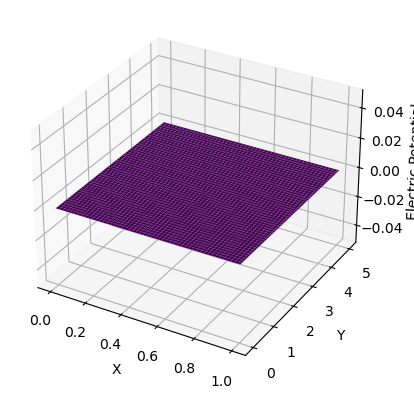
\includegraphics[keepaspectratio,alt={png}]{../images/activity-sep_var_activity-sep_var_tmp_15_1.png}}
\caption{png}
\end{figure}

\begin{Shaded}
\begin{Highlighting}[]

\end{Highlighting}
\end{Shaded}
